% ARCHITECTURE_LEGACY.tex — Architecture of the Legacy XBoing Codebase (1993–1996)
% Primary reference: docs/SPECIFICATION.md
% Author: Generated for Punt Labs modernization project

\documentclass[11pt,a4paper]{article}

% --- Encoding and typography ---
\usepackage[utf8]{inputenc}
\usepackage[T1]{fontenc}
\usepackage{microtype}
\usepackage{lmodern}

% --- Layout ---
\usepackage[margin=2.5cm]{geometry}
\usepackage[colorlinks=true,linkcolor=blue!60!black,citecolor=blue!60!black,urlcolor=blue!60!black]{hyperref}
\usepackage{amsmath}
\usepackage{cleveref}

% --- Tables ---
\usepackage{booktabs}
\usepackage{tabularx}
\usepackage{longtable}
\usepackage{array}

% --- Lists ---
\usepackage{enumitem}
\setlist{nosep,leftmargin=1.5em}

% --- Code ---
\usepackage{listings}
\lstset{
  language=C,
  basicstyle=\ttfamily\small,
  keywordstyle=\bfseries,
  commentstyle=\itshape\color{gray},
  stringstyle=\color{gray!80!black},
  showstringspaces=false,
  breaklines=true,
  frame=single,
  framesep=3pt,
  xleftmargin=6pt,
  xrightmargin=6pt,
  numbers=none,
  aboveskip=6pt,
  belowskip=6pt,
  columns=flexible,
}

% --- TikZ ---
\usepackage{tikz}
\usetikzlibrary{arrows.meta,positioning,shapes.geometric,calc,fit,backgrounds}

% --- Custom commands ---
\newcommand{\code}[1]{\texttt{#1}}
\newcommand{\file}[1]{\texttt{#1}}
\newcommand{\func}[1]{\texttt{#1()}}
\newcommand{\const}[1]{\texttt{#1}}
\newcommand{\xboing}{\textsc{XBoing}}
\newcommand{\specref}[1]{(Spec~\S#1)}

% --- Title ---
\title{\LARGE Architecture of the Legacy \xboing{} Codebase\\[6pt]
       \large X11 Breakout Game, 1993--1996}
\author{Punt Labs --- XBoing Modernization Project}
\date{May 2026 \quad\textbar\quad Revision 1.1}

\begin{document}
\maketitle

% --- Revision History ---
\noindent
\begin{tabularx}{\textwidth}{llX}
\toprule
\textbf{Rev} & \textbf{Date} & \textbf{Description} \\
\midrule
1.0 & 2026-03-24 & Initial legacy architecture document \\
1.1 & 2026-05-30 & Fact-check against \file{original/} source: corrected line counts, window dimensions, function names, constants, file inventory \\
\bottomrule
\end{tabularx}

\vspace{1em}
\tableofcontents
\newpage

% ============================================================================
\section{Introduction}
\label{sec:introduction}
% ============================================================================

\xboing{} is an X11 breakout-style game written by Justin C.\ Kibell between 1993 and 1996. It was distributed through the X Consortium under a permissive license. The game targets Unix workstations running the X Window System with PseudoColor visuals---the dominant display configuration of early-1990s SPARC, SGI, and HP-UX machines.

The codebase consists of 29 C source files (18,606 lines excluding tests), 33 headers (2,953 lines), and 12 platform-specific audio drivers (2,882 lines). It links against \code{libXpm}, \code{libX11}, and \code{libm}. There is no external game engine, framework, or toolkit; the author built directly on top of raw Xlib.

This document records the legacy architecture in sufficient detail for two audiences:
\begin{enumerate}[label=\arabic*.]
  \item \textbf{Contributors} who need to understand the original design before modifying the modernized version.
  \item \textbf{Researchers} studying AI-assisted modernization of legacy C code, who need a ``before'' baseline to compare against the SDL2-based ``after.''
\end{enumerate}

All section references marked \specref{N} point to the corresponding section in \file{docs/SPECIFICATION.md}.

% ============================================================================
\section{Build System}
\label{sec:build-system}
% ============================================================================

\subsection{Toolchain and Flags}
\label{sec:build-flags}

The original build used \code{Imakefile} (X Consortium's build generator) to produce a platform-specific \file{Makefile}. The modernized legacy build uses a hand-written \file{Makefile} with the settings in \cref{tab:build-flags}.

\begin{table}[htbp]
\centering
\caption{Compiler and linker configuration.}
\label{tab:build-flags}
\begin{tabularx}{\textwidth}{lX}
\toprule
\textbf{Setting} & \textbf{Value} \\
\midrule
Compiler     & \code{gcc} \\
CFLAGS       & \code{-O2 -Wall -Wno-unused-result -Wno-format-overflow -Wno-format-truncation} \\
Include paths & \code{-I./include -I/usr/include/X11} \\
Libraries    & \code{-lXpm -lX11 -lm} \\
\bottomrule
\end{tabularx}
\end{table}

Three warning suppressions are required because the original code uses \func{sprintf} with unchecked return values and fixed-size buffers throughout.

\subsection{Compile-Time Defines}
\label{sec:compile-defines}

All file system paths are baked in at compile time via \code{-D} flags (\cref{tab:compile-defines}). Each has a corresponding runtime environment variable override.

\begin{table}[htbp]
\centering
\caption{Compile-time defines and their runtime overrides \specref{1}.}
\label{tab:compile-defines}
\begin{tabularx}{\textwidth}{llX}
\toprule
\textbf{Define} & \textbf{Default} & \textbf{Env Override} \\
\midrule
\const{HIGH\_SCORE\_FILE}    & \code{./.xboing.scr}       & \code{XBOING\_SCORE\_FILE} \\
\const{LEVEL\_INSTALL\_DIR}  & \code{../levels}           & \code{XBOING\_LEVELS\_DIR} \\
\const{SOUNDS\_DIR}          & \code{../sounds}           & \code{XBOING\_SOUND\_DIR} \\
\const{READMEP\_FILE}        & \code{./docs/problems.doc} & --- \\
\const{AUDIO\_AVAILABLE}     & \code{True}                & --- \\
\const{AUDIO\_FILE}          & \code{audio/LINUXaudio.c}  & --- \\
\bottomrule
\end{tabularx}
\end{table}

The original source used a \const{NeedFunctionPrototypes} guard for dual K\&R / ANSI prototype support---every public function declaration was wrapped in \code{\#if NeedFunctionPrototypes} conditionals, a pattern common in X Consortium code of this era. These guards have been removed from the archived source.

\subsection{Generated Files}
\label{sec:generated-files}

Two files are generated during build:

\begin{description}[style=nextline]
  \item[\file{version.c}] Produced by \file{version.sh}. Contains four symbols: \code{dateString} (build timestamp), \code{whoString} (build user), \code{machineString} (architecture from \code{uname~-a}), and \code{buildNum} (auto-incrementing counter stored in \file{.version}).
  \item[\file{audio.c}] A symlink to the active audio driver, defaulting to \file{audio/LINUXaudio.c}. Swapping the symlink target was the mechanism for cross-platform audio.
\end{description}

\subsection{Source File Inventory}
\label{sec:source-inventory}

The build compiles 29 \file{.c} files (listed in \cref{tab:source-files}) and links them into a single \code{xboing} binary.

\begin{longtable}{lrl}
\caption{Source files with line counts (excluding tests and stubs).}
\label{tab:source-files} \\
\toprule
\textbf{File} & \textbf{Lines} & \textbf{Role} \\
\midrule
\endfirsthead
\toprule
\textbf{File} & \textbf{Lines} & \textbf{Role} \\
\midrule
\endhead
\file{blocks.c}    & 2,631 & Block grid, 30 types, collision regions \\
\file{ball.c}      & 2,099 & Ball physics, collision detection \\
\file{main.c}      & 1,768 & Event loop, state machine, input \\
\file{editor.c}    & 1,198 & Level editor \\
\file{init.c}      & 1,071 & X11 setup, colormap, fonts \\
\file{highscore.c} & 1,065 & Score file I/O, display \\
\file{bonus.c}     &   775 & Bonus sequence \\
\file{presents.c}  &   701 & Credits/splash sequence \\
\file{file.c}      &   703 & Level file parsing, save/load \\
\file{gun.c}       &   642 & Bullet system \\
\file{stage.c}     &   581 & Window hierarchy creation \\
\file{level.c}     &   511 & Level management, timer \\
\file{misc.c}      &   499 & Drawing utilities \\
\file{intro.c}     &   469 & Introduction screen \\
\file{eyedude.c}   &   402 & Animated enemy character \\
\file{dialogue.c}  &   393 & Modal input dialogs \\
\file{sfx.c}       &   383 & Visual special effects \\
\file{keys.c}      &   384 & Key bindings display \\
\file{paddle.c}    &   357 & Paddle control \\
\file{demo.c}      &   340 & Demo mode \\
\file{keysedit.c}  &   327 & Editor key bindings display \\
\file{inst.c}      &   287 & Instructions screen \\
\file{special.c}   &   253 & Power-up state management \\
\file{preview.c}   &   241 & Level preview screen \\
\file{score.c}     &   219 & Score digit display \\
\file{mess.c}      &   159 & Message bar \\
\file{error.c}     &   148 & Error/warning output \\
\file{version.c}   &     --- & Generated (build metadata) \\
\file{audio.c}     &     --- & Symlink to platform driver \\
\midrule
\textbf{Total}     & \textbf{18,606} & (27 files, excl.\ generated) \\
\bottomrule
\end{longtable}

% ============================================================================
\section{Window System and Graphics}
\label{sec:graphics}
% ============================================================================

\subsection{X11 Initialization Sequence}
\label{sec:x11-init}

\func{InitialiseGame} in \file{init.c} performs 33 ordered initialization steps \specref{16}. The sequence has implicit dependencies: colormap must precede color allocation, which must precede window creation, which must precede GC creation. Reordering any step risks segfaults or blank windows.

The visual selection algorithm tries, in order: PseudoColor, DirectColor, TrueColor. PseudoColor was the norm on 1993 workstations; modern systems universally provide TrueColor.

\subsection{Window Hierarchy}
\label{sec:window-hierarchy}

The application creates 11 windows: one top-level \code{mainWindow} and 10 child windows for distinct UI regions (\cref{tab:windows}). This was standard Xlib practice---each sub-window provides its own clipping rectangle, event routing, and background.

\begin{table}[htbp]
\centering
\caption{Window hierarchy with positions and dimensions \specref{2}.}
\label{tab:windows}
\begin{tabularx}{\textwidth}{lllX}
\toprule
\textbf{Window} & \textbf{Size (px)} & \textbf{Position} & \textbf{Purpose} \\
\midrule
\code{mainWindow}    & 575 $\times$ 720 & (0,0)    & Top-level container \\
\code{playWindow}    & 495 $\times$ 580 & (35,60)  & Gameplay area \\
\code{bufferWindow}  & 495 $\times$ 580 & (35,60)  & Offscreen double buffer \\
\code{scoreWindow}   & 224 $\times$ 42  & (35,10)  & Score display \\
\code{levelWindow}   & 286 $\times$ 52  & (284,5)  & Level, lives, ammo \\
\code{messWindow}    & 247 $\times$ 30  & (35,655) & Status messages \\
\code{specialWindow} & 180 $\times$ 35  & (292,655) & Active specials \\
\code{timeWindow}    & 61 $\times$ 35   & (477,655) & Timer display \\
\code{blockWindow}   & 120 $\times$ 580 & (545,60) & Editor palette \\
\code{typeWindow}    & 120 $\times$ 35  & (545,650) & Editor block type \\
\code{inputWindow}   & 380 $\times$ 120 & (92,295)  & Modal input dialog \\
\bottomrule
\end{tabularx}
\end{table}

The \code{bufferWindow} is never mapped (made visible). It serves as an offscreen pixmap for double buffering---SFX transitions copy from \code{bufferWindow} to \code{playWindow} in strips or chunks.

\begin{figure}[htbp]
\centering
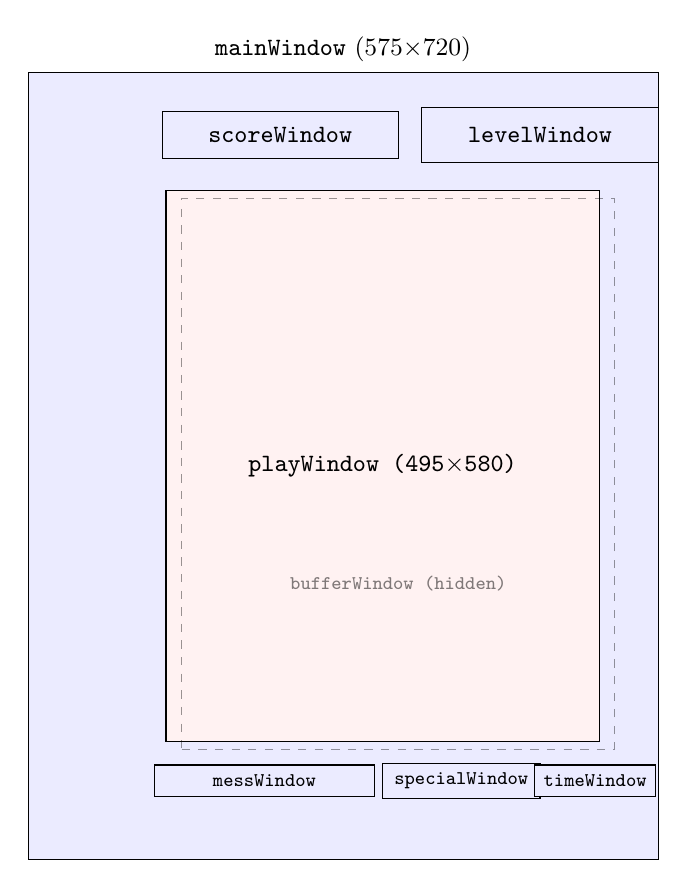
\begin{tikzpicture}[
  win/.style={draw, minimum height=1cm, fill=blue!8, font=\small\ttfamily},
  arr/.style={-{Stealth[length=3pt]}, thick}
]
  % Main window
  \node[win, minimum width=8cm, minimum height=10cm] (main) {};
  \node[above] at (main.north) {\small\texttt{mainWindow} (575$\times$720)};

  % Score and Level windows at top
  \node[win, minimum width=3cm, minimum height=0.6cm] at (-0.8, 4.2) (score) {scoreWindow};
  \node[win, minimum width=3cm, minimum height=0.7cm] at (2.5, 4.2) (level) {levelWindow};

  % Play area
  \node[win, minimum width=5.5cm, minimum height=7cm, fill=red!5] at (0.5, 0) (play) {};
  \node[font=\small\ttfamily] at (0.5, 0) {playWindow (495$\times$580)};

  % Buffer (dashed - hidden)
  \node[draw, dashed, minimum width=5.5cm, minimum height=7cm, opacity=0.4] at (0.7, -0.1) (buf) {};
  \node[font=\scriptsize\ttfamily, opacity=0.5] at (0.7, -1.5) {bufferWindow (hidden)};

  % Bottom windows
  \node[win, minimum width=2.8cm, minimum height=0.4cm] at (-1.0, -4.0) (mess) {\scriptsize messWindow};
  \node[win, minimum width=2cm, minimum height=0.4cm] at (1.5, -4.0) (spec) {\scriptsize specialWindow};
  \node[win, minimum width=0.8cm, minimum height=0.4cm] at (3.2, -4.0) (time) {\scriptsize timeWindow};

\end{tikzpicture}
\caption{X11 window hierarchy. The \texttt{bufferWindow} (dashed) is an unmapped offscreen surface used for SFX compositing. Editor windows (\texttt{blockWindow}, \texttt{typeWindow}) omitted---they extend the main window width when the editor is active.}
\label{fig:window-hierarchy}
\end{figure}

\subsection{Graphics Contexts}
\label{sec:gcs}

Six GCs control all drawing operations (\cref{tab:gcs}). The X11 GC is a server-side object that stores drawing parameters (function, foreground/background, fill style, clip mask). Switching drawing modes requires selecting a different GC, not modifying one in place.

\begin{table}[htbp]
\centering
\caption{Graphics contexts and their X11 raster operations \specref{2}.}
\label{tab:gcs}
\begin{tabular}{llll}
\toprule
\textbf{GC} & \textbf{X Function} & \textbf{Fill Style} & \textbf{Purpose} \\
\midrule
\code{gccopy} & \code{GXcopy}  & Solid     & Standard blitting \\
\code{gc}     & \code{GXcopy}  & FillTiled & Tiled pattern fills \\
\code{gcxor}  & \code{GXxor}   & Solid     & Reversible drawing (erase by redraw) \\
\code{gcand}  & \code{GXand}   & Solid     & Mask application (fg=0, bg=$\sim$0) \\
\code{gcor}   & \code{GXor}    & Solid     & Image compositing (OR combine) \\
\code{gcsfx}  & \code{GXcopy}  & Solid     & Special effects \\
\bottomrule
\end{tabular}
\end{table}

The AND/OR pair implements sprite transparency: AND the mask (clearing the sprite area), then OR the sprite image (compositing it onto the background). This three-step blit pattern predates alpha blending.

\subsection{XPM Pixmap Loading and Rendering Pipeline}
\label{sec:rendering-pipeline}

All graphics are XPM files---a C-header format encoding indexed-color images. The \func{XpmCreatePixmapFromData} function (from \code{libXpm}) returns both a \code{Pixmap} (image data) and a shape \code{Pixmap} (1-bit transparency mask). The rendering pipeline is:

\begin{figure}[htbp]
\centering
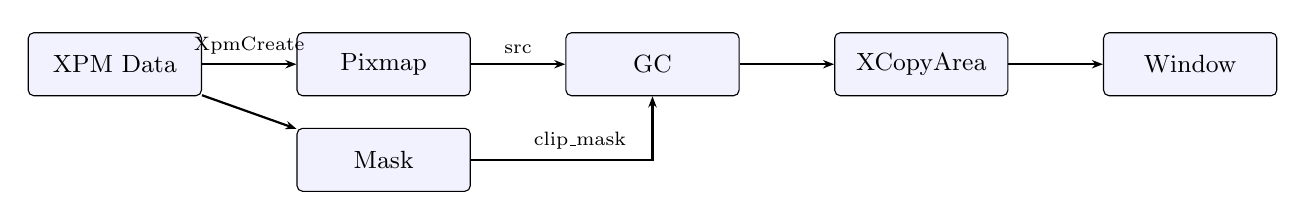
\begin{tikzpicture}[
  box/.style={draw, rounded corners=2pt, minimum height=0.8cm, minimum width=2.2cm, font=\small, fill=blue!5},
  arr/.style={-{Stealth[length=4pt]}, thick},
  lbl/.style={font=\scriptsize, midway, above}
]
  \node[box] (xpm) {XPM Data};
  \node[box, right=1.2cm of xpm] (pix) {Pixmap};
  \node[box, below=0.4cm of pix] (mask) {Mask};
  \node[box, right=1.2cm of pix] (gc) {GC};
  \node[box, right=1.2cm of gc] (copy) {XCopyArea};
  \node[box, right=1.2cm of copy] (win) {Window};

  \draw[arr] (xpm) -- node[lbl] {\scriptsize XpmCreate} (pix);
  \draw[arr] (xpm) -- (mask);
  \draw[arr] (mask) -| node[lbl,pos=0.3] {\scriptsize clip\_mask} (gc);
  \draw[arr] (pix) -- node[lbl] {\scriptsize src} (gc);
  \draw[arr] (gc) -- (copy);
  \draw[arr] (copy) -- (win);
\end{tikzpicture}
\caption{Rendering pipeline: XPM source $\to$ Pixmap + Mask $\to$ GC with clip mask $\to$ XCopyArea $\to$ destination Window.}
\label{fig:rendering-pipeline}
\end{figure}

\subsection{Colormap and Color Cycling}
\label{sec:colormap}

The game allocates a private PseudoColor colormap with 8 named colors (red, tan, yellow, green, purple, blue, white, black) and two cycling arrays:

\begin{itemize}
  \item \code{reds[7]}: shades from \code{\#f00} to \code{\#300} (indices 0--6)
  \item \code{greens[7]}: shades from \code{\#0f0} to \code{\#030} (indices 0--6)
\end{itemize}

These arrays drive the border glow animation, which cycles every 40 frames. When the \code{noWalls} power-up is active, the border switches to the green array.

\subsection{Font Handling}
\label{sec:fonts}

Four Adobe Helvetica bitmap fonts are loaded via XLFD (X Logical Font Description) patterns (\cref{tab:fonts}). If any pattern fails to match, the code falls back to the \code{"fixed"} font.

\begin{table}[htbp]
\centering
\caption{Font specifications \specref{2}.}
\label{tab:fonts}
\begin{tabular}{llll}
\toprule
\textbf{Variable} & \textbf{Size} & \textbf{Weight} & \textbf{Usage} \\
\midrule
\code{titleFont} & 24pt & Bold   & Title text \\
\code{textFont}  & 18pt & Medium & General text \\
\code{dataFont}  & 14pt & Bold   & Data and intro text \\
\code{copyFont}  & 12pt & Medium & Copyright, specials \\
\bottomrule
\end{tabular}
\end{table}

\subsection{SFX Compositing}
\label{sec:sfx-compositing}

Five visual effects use the \code{bufferWindow} as a source and \code{playWindow} as a destination (\cref{tab:sfx}). All require backing store (\code{DoesBackingStore() == Always}); without it, effects are silently disabled.

\begin{table}[htbp]
\centering
\caption{Visual special effects modes \specref{10}.}
\label{tab:sfx}
\begin{tabularx}{\textwidth}{lllX}
\toprule
\textbf{ID} & \textbf{Constant} & \textbf{Name} & \textbf{Technique} \\
\midrule
1 & \const{SFX\_SHAKE}   & Shake   & Move \code{playWindow} $\pm$3\,px randomly every 5 frames \\
2 & \const{SFX\_FADE}    & Fade    & Draw black grid lines at 12\,px spacing \\
3 & \const{SFX\_BLIND}   & Blind   & Copy buffer in 8 vertical strips \\
4 & \const{SFX\_SHATTER} & Shatter & 10$\times$10 scatter grid, randomized chunk copy \\
5 & \const{SFX\_STATIC}  & Static  & Placeholder (no animation) \\
\bottomrule
\end{tabularx}
\end{table}


% ============================================================================
\section{Audio System}
\label{sec:audio}
% ============================================================================

\subsection{Fork+Pipe Architecture}
\label{sec:audio-arch}

The audio system uses a Unix process model: \func{SetUpAudioSystem} calls \func{fork} to create a child process. Parent and child communicate over a unidirectional pipe. The parent writes sound file names (null-terminated strings) to the pipe; the child reads them, opens the corresponding \file{.au} file, and writes raw PCM data to \file{/dev/dsp} via the OSS (Open Sound System) interface.

\begin{figure}[htbp]
\centering
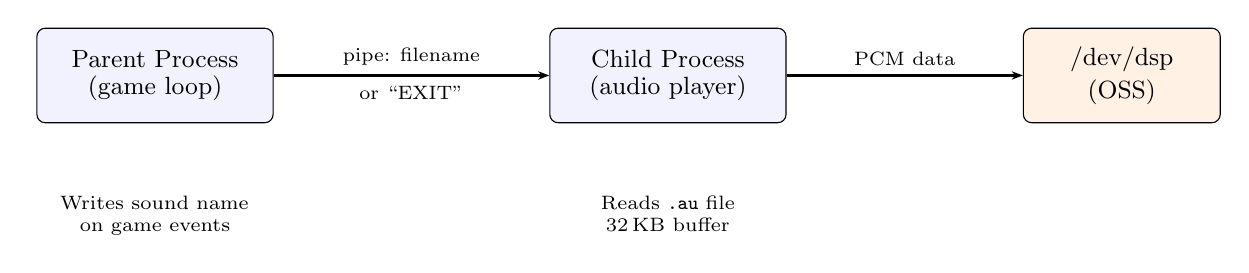
\begin{tikzpicture}[
  proc/.style={draw, rounded corners=3pt, minimum height=1.2cm, minimum width=3cm, font=\small, fill=blue!5},
  dev/.style={draw, rounded corners=3pt, minimum height=1.2cm, minimum width=2.5cm, font=\small, fill=orange!10},
  arr/.style={-{Stealth[length=4pt]}, thick},
]
  \node[proc] (parent) {\shortstack{Parent Process\\(game loop)}};
  \node[proc, right=3.5cm of parent] (child) {\shortstack{Child Process\\(audio player)}};
  \node[dev, right=3cm of child] (dsp) {\shortstack{/dev/dsp\\(OSS)}};

  \draw[arr] (parent) -- node[above, font=\scriptsize] {pipe: filename} node[below, font=\scriptsize] {or ``EXIT''} (child);
  \draw[arr] (child) -- node[above, font=\scriptsize] {PCM data} (dsp);

  \node[below=0.8cm of parent, font=\scriptsize, text width=3cm, align=center] {Writes sound name\\on game events};
  \node[below=0.8cm of child, font=\scriptsize, text width=3cm, align=center] {Reads \texttt{.au} file\\32\,KB buffer};
\end{tikzpicture}
\caption{Audio fork+pipe architecture. The child process blocks on pipe reads when idle. Termination is signaled by writing the string ``EXIT.''}
\label{fig:audio-arch}
\end{figure}

The 32\,KB buffer (\const{SBUF\_SIZE} = 32, \const{BUFFER\_SIZE} = 1024 $\times$ 32) is used for reading \file{.au} file data. After playing each file, the child issues \code{SNDCTL\_DSP\_SYNC} to flush the device. Volume control is a no-op in the Linux driver.

\subsection{Platform Drivers}
\label{sec:audio-drivers}

Twelve drivers exist in the \file{audio/} directory (\cref{tab:audio-drivers}). The active driver is selected at build time by creating the \file{audio.c} symlink. All drivers implement the same 6-function API: \func{SetUpAudioSystem}, \func{FreeAudioSystem}, \func{playSoundFile}, \func{audioDeviceEvents}, \func{SetMaximumVolume}, \func{GetMaximumVolume}.

\begin{table}[htbp]
\centering
\caption{Audio driver inventory (2,882 lines total) \specref{3}.}
\label{tab:audio-drivers}
\begin{tabular}{llr}
\toprule
\textbf{Driver File} & \textbf{Platform} & \textbf{Lines} \\
\midrule
\file{LINUXaudio.c}  & Linux OSS (\file{/dev/dsp})    & 234 \\
\file{LINUXaudio2.c} & Linux alternate                 & 292 \\
\file{ALSAaudio.c}   & ALSA                            & 76 \\
\file{SUNaudio.c}    & SunOS/Solaris                   & 389 \\
\file{SGIaudio.c}    & SGI IRIX                        & 305 \\
\file{HPaudio.c}     & HP-UX                           & 200 \\
\file{BSDaudio.c}    & BSD                             & 323 \\
\file{SVR4audio.c}   & System V Release 4              & 222 \\
\file{AFaudio.c}     & AudioFile (AF) protocol         & 322 \\
\file{RPLAYaudio.c}  & RPLAY (remote audio)            & 187 \\
\file{NCDaudio.c}    & Network Computing Devices       & 229 \\
\file{NOaudio.c}     & Null/silent                     & 103 \\
\bottomrule
\end{tabular}
\end{table}

\subsection{Sound Assets}
\label{sec:sound-assets}

The game ships 46 \file{.au} (Sun Audio) files in \file{sounds/}. Sound names are passed as bare strings (e.g., \code{"boing"}, \code{"applause"}) and the driver constructs the full path as \code{\{SOUNDS\_DIR\}/\{name\}.au}.


% ============================================================================
\section{Game State Machine}
\label{sec:state-machine}
% ============================================================================

\subsection{Mode Enumeration}
\label{sec:modes}

The game has 16 modes, defined as integer constants in \file{main.h} (\cref{tab:modes}). The active mode is stored in the global variable \code{mode}; the previous mode in \code{oldMode}.

\begin{table}[htbp]
\centering
\caption{Game mode constants \specref{4}.}
\label{tab:modes}
\begin{tabular}{rll}
\toprule
\textbf{ID} & \textbf{Constant} & \textbf{Description} \\
\midrule
0  & \const{MODE\_NONE}      & Uninitialized \\
1  & \const{MODE\_HIGHSCORE} & High score display \\
2  & \const{MODE\_INTRO}     & Introduction/splash \\
3  & \const{MODE\_GAME}      & Active gameplay \\
4  & \const{MODE\_PAUSE}     & Paused \\
5  & \const{MODE\_BALL\_WAIT}& Waiting for ball activation \\
6  & \const{MODE\_WAIT}      & Generic wait \\
7  & \const{MODE\_BONUS}     & Level-complete bonus sequence \\
8  & \const{MODE\_INSTRUCT}  & Instructions display \\
9  & \const{MODE\_KEYS}      & Key bindings display \\
10 & \const{MODE\_PRESENTS}  & Credits/splash (startup) \\
11 & \const{MODE\_DEMO}      & Auto-play demo \\
12 & \const{MODE\_PREVIEW}   & Level preview \\
13 & \const{MODE\_DIALOGUE}  & Modal dialog \\
14 & \const{MODE\_EDIT}      & Level editor \\
15 & \const{MODE\_KEYSEDIT}  & Editor key bindings \\
\bottomrule
\end{tabular}
\end{table}

\subsection{State Transition Diagram}
\label{sec:state-transitions}

\begin{figure}[htbp]
\centering
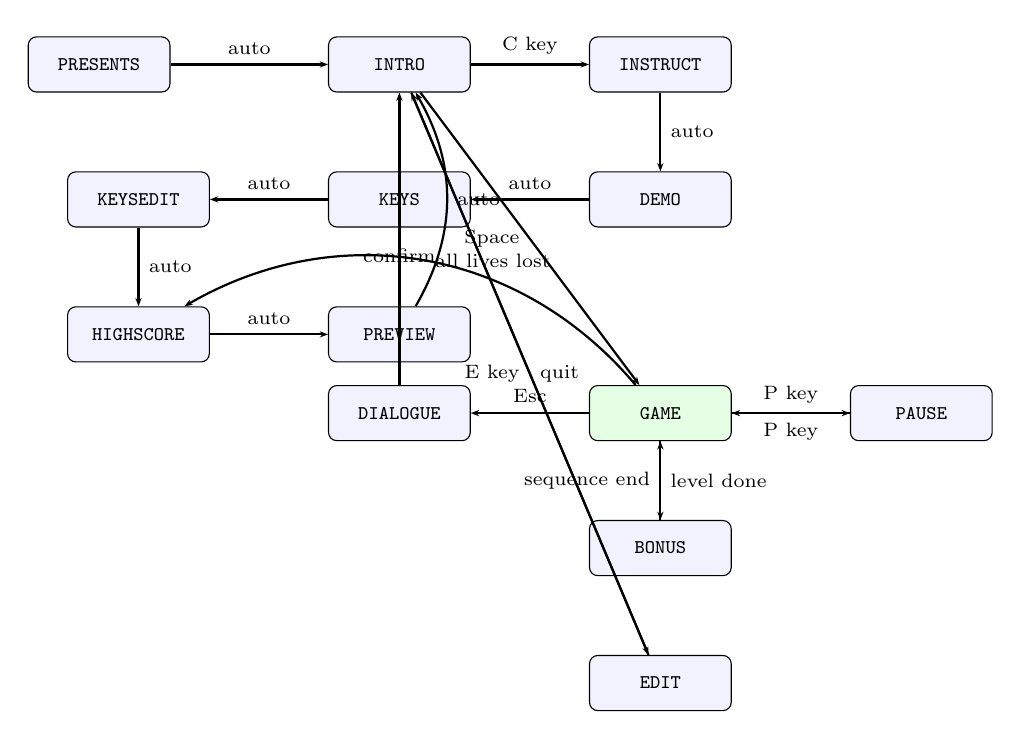
\begin{tikzpicture}[
  state/.style={draw, rounded corners=3pt, minimum height=0.7cm, minimum width=1.8cm, font=\scriptsize\ttfamily, fill=blue!5},
  trans/.style={-{Stealth[length=3pt]}, thick, font=\scriptsize},
  node distance=1.2cm and 1.5cm,
]
  % Startup
  \node[state] (presents) {PRESENTS};
  \node[state, right=2cm of presents] (intro) {INTRO};
  \node[state, right=1.5cm of intro] (instruct) {INSTRUCT};
  \node[state, below=1cm of instruct] (demo) {DEMO};
  \node[state, left=1.5cm of demo] (keys) {KEYS};
  \node[state, left=1.5cm of keys] (keysedit) {KEYSEDIT};
  \node[state, below=1cm of keysedit] (highscore) {HIGHSCORE};
  \node[state, right=1.5cm of highscore] (preview) {PREVIEW};

  % Menu cycle
  \draw[trans] (presents) -- node[above] {auto} (intro);
  \draw[trans] (intro) -- node[above] {C key} (instruct);
  \draw[trans] (instruct) -- node[right] {auto} (demo);
  \draw[trans] (demo) -- node[above] {auto} (keys);
  \draw[trans] (keys) -- node[above] {auto} (keysedit);
  \draw[trans] (keysedit) -- node[right] {auto} (highscore);
  \draw[trans] (highscore) -- node[above] {auto} (preview);
  \draw[trans] (preview) to[bend right=30] node[right, font=\scriptsize] {auto} (intro);

  % Gameplay cluster
  \node[state, below=2cm of demo, fill=green!10] (game) {GAME};
  \node[state, right=1.5cm of game] (pause) {PAUSE};
  \node[state, below=1cm of game] (bonus) {BONUS};
  \node[state, left=1.5cm of game] (dialogue) {DIALOGUE};
  \node[state, below=1cm of bonus] (edit) {EDIT};

  % Gameplay transitions
  \draw[trans] (intro) -- node[left, font=\scriptsize] {Space} (game);
  \draw[trans] (game) -- node[above] {P key} (pause);
  \draw[trans] (pause) -- node[below] {P key} (game);
  \draw[trans] (game) -- node[right] {level done} (bonus);
  \draw[trans] (bonus) -- node[left] {sequence end} (game);
  \draw[trans] (game) -- node[above] {Esc} (dialogue);
  \draw[trans] (dialogue) -- node[below, font=\scriptsize] {confirm} (intro);
  \draw[trans] (game) to[bend right=40] node[right, font=\scriptsize] {all lives lost} (highscore);
  \draw[trans] (intro) -- node[left, font=\scriptsize] {E key} (edit);
  \draw[trans] (edit) -- node[right, font=\scriptsize] {quit} (intro);
\end{tikzpicture}
\caption{Game state machine. Green node = active gameplay. Menu modes (top) cycle automatically via the C key or frame-count timeouts. Gameplay modes (bottom) are entered from any menu mode via Space.}
\label{fig:state-machine}
\end{figure}

\subsection{Event Loop}
\label{sec:event-loop}

The event loop in \func{handleEventLoop} (\file{main.c}) runs a non-blocking poll during gameplay and a blocking wait during pause or iconification:

\begin{lstlisting}[caption={Event loop structure (simplified).}]
void handleEventLoop(Display *display) {
    /* Wait for MapNotify, grab pointer */
    while (True) {
        audioDeviceEvents();
        if (!iconified && mode != MODE_PAUSE) {
            XPending(display);      /* non-blocking */
            if (mode != MODE_DIALOGUE) frame++;
        } else {
            XPeekEvent(display, &event);  /* blocks */
            XPending(display);
        }
        /* dispatch: KeyPress, ButtonPress, Expose, Map/Unmap */
        if (!iconified) {
            if (mode == MODE_GAME || mode == MODE_BALL_WAIT)
                sleepSync(display, speed);
            else
                sleepSync(display, 3);
            handleGameStates(display);
        }
    }
}
\end{lstlisting}

\func{sleepSync} calls \code{XSync(display, False)} followed by \code{usleep(ms * 300)}. The 300$\times$ multiplier was hand-tuned for mid-1990s workstation performance.

\subsection{Frame Timing}
\label{sec:frame-timing}

Three speed constants define the base timing (\cref{tab:timing}). Speed keys 1--9 adjust \code{userDelay}: key~1 sets delay~9 (slowest), key~9 sets delay~1 (fastest).

\begin{table}[htbp]
\centering
\caption{Frame timing constants \specref{4}.}
\label{tab:timing}
\begin{tabular}{llr}
\toprule
\textbf{Constant} & \textbf{Value} & \textbf{Effective Sleep ($\mu$s)} \\
\midrule
\const{FAST\_SPEED}   & 5\,ms  & 1,500 \\
\const{MEDIUM\_SPEED} & 15\,ms & 4,500 \\
\const{SLOW\_SPEED}   & 30\,ms & 9,000 \\
\bottomrule
\end{tabular}
\end{table}

% ============================================================================
\section{Ball Physics and Collision}
\label{sec:ball-physics}
% ============================================================================

\subsection{Ball Data Structure}
\label{sec:ball-struct}

Each ball is represented by a \code{BALL} struct (\cref{tab:ball-struct}). The game supports up to \const{MAX\_BALLS} = 5 simultaneous balls.

\begin{table}[htbp]
\centering
\caption{Ball structure fields \specref{5}.}
\label{tab:ball-struct}
\begin{tabularx}{\textwidth}{llX}
\toprule
\textbf{Field} & \textbf{Type} & \textbf{Description} \\
\midrule
\code{ballx}, \code{bally}       & \code{int}   & Current center position (pixels) \\
\code{oldx}, \code{oldy}         & \code{int}   & Previous position \\
\code{dx}, \code{dy}             & \code{int}   & Velocity components (px/frame) \\
\code{radius}                     & \code{float} & Geometric radius \\
\code{mass}                       & \code{float} & Mass (1.0--3.0) \\
\code{active}                     & \code{int}   & True if ball in use \\
\code{ballState}                  & enum         & Current state (8 values, see \cref{sec:ball-states}) \\
\code{slide}                      & \code{int}   & Animation frame index (0--4) \\
\code{lastPaddleHitFrame}         & \code{int}   & Frame of last paddle contact \\
\code{waitMode}, \code{waitingFrame}, \code{newMode} & various & Wait/transition control \\
\bottomrule
\end{tabularx}
\end{table}

Key constants: \const{BALL\_WIDTH} = 20\,px, \const{BALL\_HEIGHT} = 19\,px, \const{MAX\_X\_VEL} = \const{MAX\_Y\_VEL} = 14\,px/frame, \const{MIN\_DX\_BALL} = \const{MIN\_DY\_BALL} = 2\,px/frame.

\subsection{Ball State Machine}
\label{sec:ball-states}

\begin{table}[htbp]
\centering
\caption{Ball states and lifecycle \specref{5}.}
\label{tab:ball-states}
\begin{tabular}{rll}
\toprule
\textbf{Value} & \textbf{State} & \textbf{Description} \\
\midrule
0 & \const{BALL\_POP}    & Dying animation (8 frames) \\
1 & \const{BALL\_ACTIVE} & In play, moving \\
2 & \const{BALL\_STOP}   & Dead \\
3 & \const{BALL\_CREATE} & Birth animation (8 frames) \\
4 & \const{BALL\_DIE}    & About to die \\
5 & \const{BALL\_WAIT}   & Transitioning between modes \\
6 & \const{BALL\_READY}  & On paddle, awaiting launch \\
7 & \const{BALL\_NONE}   & Null/unused \\
\bottomrule
\end{tabular}
\end{table}

Lifecycle: \const{BALL\_NONE} $\to$ \const{BALL\_CREATE} (8-frame birth) $\to$ \const{BALL\_READY} (auto-launch after 3,000\,ms) $\to$ \const{BALL\_ACTIVE} $\to$ \const{BALL\_DIE}/\const{BALL\_POP} (8-frame death) $\to$ \const{BALL\_NONE}.

\subsection{Paddle Collision and Bounce Angle}
\label{sec:paddle-collision}

The ball-paddle collision test is a geometric line intersection. The paddle sits at $y = \text{PLAY\_HEIGHT} - \text{DIST\_BASE} - 2$ (where \const{DIST\_BASE} = 30). Two cases:

\textbf{Case A} (vertical ball, $dx = 0$): check if \code{ballx} falls within paddle bounds.

\textbf{Case B} (diagonal ball, $dx \neq 0$): compute the trajectory line $y = \alpha x + \beta$, find the intersection $x_H = (\text{paddleLine} - \beta) / \alpha$, and check if $x_H$ is within paddle bounds.

The bounce angle uses trigonometric reflection:
\begin{align}
  V_s &= \sqrt{V_x^2 + V_y^2} \label{eq:speed} \\
  \alpha &= \arctan\!\left(\frac{V_x}{-V_y}\right) \label{eq:angle} \\
  \beta &= \arctan\!\left(\frac{\text{hitPos}}{\text{padSize}}\right) \label{eq:reflect} \\
  \gamma &= 2\beta - \alpha \label{eq:new-angle} \\
  V_x' &= V_s \sin\gamma + \frac{\text{paddleDx}}{10} \label{eq:vx} \\
  V_y' &= -V_s \cos\gamma \label{eq:vy}
\end{align}

The term $\text{paddleDx}/10$ in \cref{eq:vx} adds paddle momentum to the ball, allowing the player to influence ball direction through paddle movement. Minimum upward velocity is enforced: $dy' \geq -\text{MIN\_DY\_BALL}$.

\subsection{Block Collision (4-Region System)}
\label{sec:block-collision}

Each block is divided into 4 triangular collision regions using \func{XPolygonRegion}. The ball's bounding box is tested against each region via \func{XRectInRegion} to determine bounce direction.

\begin{figure}[htbp]
\centering
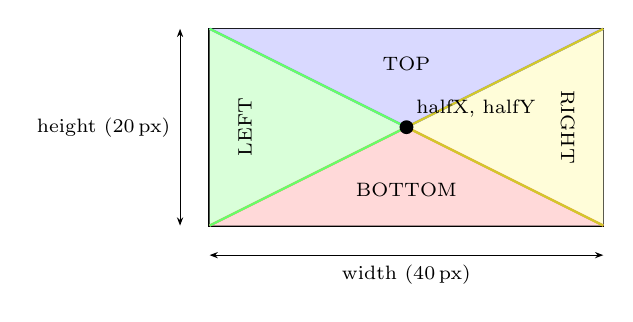
\begin{tikzpicture}[scale=2.5]
  % Block outline
  \draw[thick] (0,0) rectangle (2,1);

  % Center point
  \coordinate (center) at (1, 0.5);

  % Four triangles
  \fill[red!15] (0,0) -- (center) -- (2,0) -- cycle;
  \fill[blue!15] (0,1) -- (center) -- (2,1) -- cycle;
  \fill[green!15] (0,0) -- (center) -- (0,1) -- cycle;
  \fill[yellow!15] (2,0) -- (center) -- (2,1) -- cycle;

  % Triangle borders
  \draw[thick, red!60] (0,0) -- (center) -- (2,0);
  \draw[thick, blue!60] (0,1) -- (center) -- (2,1);
  \draw[thick, green!60] (0,0) -- (center) -- (0,1);
  \draw[thick, yellow!80!black] (2,0) -- (center) -- (2,1);

  % Labels
  \node[font=\scriptsize] at (1, 0.18) {BOTTOM};
  \node[font=\scriptsize] at (1, 0.82) {TOP};
  \node[font=\scriptsize, rotate=90] at (0.18, 0.5) {LEFT};
  \node[font=\scriptsize, rotate=-90] at (1.82, 0.5) {RIGHT};

  % Center dot
  \fill (center) circle (1pt);
  \node[font=\scriptsize, above right] at (center) {halfX, halfY};

  % Dimensions
  \draw[{Stealth[length=3pt]}-{Stealth[length=3pt]}] (0, -0.15) -- (2, -0.15) node[midway, below, font=\scriptsize] {width (40\,px)};
  \draw[{Stealth[length=3pt]}-{Stealth[length=3pt]}] (-0.15, 0) -- (-0.15, 1) node[midway, left, font=\scriptsize] {height (20\,px)};
\end{tikzpicture}
\caption{Block collision regions. Each block is divided into 4 triangles meeting at the center. The region hit determines bounce direction: TOP/BOTTOM reverses $dy$; LEFT/RIGHT reverses $dx$. Corner hits combine flags.}
\label{fig:collision-regions}
\end{figure}

Region constants: \const{REGION\_TOP} = 1, \const{REGION\_BOTTOM} = 2, \const{REGION\_LEFT} = 4, \const{REGION\_RIGHT} = 8. Corner hits combine via bitwise OR.

Detection priority depends on ball direction: if $|dx| > |dy|$, horizontal regions are checked first; otherwise, vertical regions take priority.

\subsection{Ball-to-Ball Collision}
\label{sec:ball-ball}

Ball-to-ball collision uses a quadratic prediction to find the collision time within the current frame. Given position delta $\mathbf{p}$ and velocity delta $\mathbf{v}$ between two balls:

\begin{align}
  v^2 &= v_x^2 + v_y^2 \\
  r^2 &= (r_1 + r_2)^2 \\
  D &= v^2 \cdot r^2 - (v_x p_y - v_y p_x)^2
\end{align}

If $D \geq 0$ and $v^2 > \epsilon$ (where $\epsilon = \sqrt{1.4 \times 10^{-45}}$), a collision is predicted. The collision time $t_{\min}$ is computed via the quadratic formula; if $0 \leq t_{\min} \leq 1$, collision occurs this frame.

The elastic response uses mass-based velocity exchange:
\begin{align}
  m_r &= m_1 / m_2 \\
  k &= \frac{-2(\mathbf{v} \cdot \mathbf{p})}{1 + m_r} \\
  \Delta\mathbf{v}_1 &= k \cdot \hat{\mathbf{p}}, \qquad
  \Delta\mathbf{v}_2 = -k \cdot m_r \cdot \hat{\mathbf{p}}
\end{align}

\subsection{Wall Collisions}
\label{sec:wall-collisions}

\begin{table}[htbp]
\centering
\caption{Boundary collision behavior \specref{5}.}
\label{tab:wall-collisions}
\begin{tabularx}{\textwidth}{lXX}
\toprule
\textbf{Boundary} & \textbf{Normal Mode} & \textbf{noWalls Mode} \\
\midrule
Left ($x < \text{BALL\_WC}$)   & Reverse $dx$: $dx = |dx|$   & Wrap right: $x = \text{PLAY\_WIDTH} - \text{BALL\_WC}$ \\
Right ($x > \text{PW} - \text{BALL\_WC}$)  & Reverse $dx$: $dx = -|dx|$  & Wrap left: $x = \text{BALL\_WC}$ \\
Top ($y < \text{BALL\_HC}$)    & Reverse $dy$: $dy = |dy|$   & Same (reverse $dy$) \\
Bottom ($y > \text{PH} + 2 \cdot \text{BH}$) & Ball dies & Ball dies \\
\bottomrule
\end{tabularx}
\end{table}


% ============================================================================
\section{Block System}
\label{sec:blocks}
% ============================================================================

\subsection{Grid Structure}
\label{sec:block-grid}

The block grid is an 18$\times$9 array (\const{MAX\_ROW}~$\times$~\const{MAX\_COL}) of \code{struct aBlock}. Each cell is 40$\times$20\,px (\const{BLOCK\_WIDTH}~$\times$~\const{BLOCK\_HEIGHT}), except \const{BLACK\_BLK} (50$\times$30) and \const{BOMB\_BLK}/\const{DEATH\_BLK} (30$\times$30). The bottom 3 rows are reserved for the paddle area, leaving 15 playable rows.

The \code{aBlock} struct has 29 fields including pixel position, collision regions (4 X11 \code{Region} objects), animation state, explosion state, ball hit tracking, and type-specific counters.

\subsection{Block Type Catalog}
\label{sec:block-types}

\begin{longtable}{rlcrrl}
\caption{Complete block type table (30 types) \specref{6}.}
\label{tab:block-types} \\
\toprule
\textbf{ID} & \textbf{Enum} & \textbf{Char} & \textbf{Size} & \textbf{Points} & \textbf{Behavior} \\
\midrule
\endfirsthead
\toprule
\textbf{ID} & \textbf{Enum} & \textbf{Char} & \textbf{Size} & \textbf{Points} & \textbf{Behavior} \\
\midrule
\endhead
0  & \const{RED\_BLK}         & \code{r} & 40$\times$20 & 100 & Standard \\
1  & \const{BLUE\_BLK}        & \code{b} & 40$\times$20 & 110 & Standard \\
2  & \const{GREEN\_BLK}       & \code{g} & 40$\times$20 & 120 & Standard \\
3  & \const{TAN\_BLK}         & \code{t} & 40$\times$20 & 130 & Standard \\
4  & \const{YELLOW\_BLK}      & \code{y} & 40$\times$20 & 140 & Standard \\
5  & \const{PURPLE\_BLK}      & \code{p} & 40$\times$20 & 150 & Standard \\
6  & \const{BULLET\_BLK}      & \code{B} & 40$\times$20 & 50  & Ammo pickup \\
7  & \const{BLACK\_BLK}       & \code{w} & 50$\times$30 & 0   & Indestructible wall \\
8  & \const{COUNTER\_BLK}     & \code{0--5} & 40$\times$20 & 200 & Multi-hit (0--5) \\
9  & \const{BOMB\_BLK}        & \code{X} & 30$\times$30 & 50  & Chain explosion \\
10 & \const{DEATH\_BLK}       & \code{D} & 30$\times$30 & 0   & Instant ball kill \\
11 & \const{REVERSE\_BLK}     & \code{R} & 33$\times$16 & 100 & Reverse controls \\
12 & \const{HYPERSPACE\_BLK}  & \code{H} & 31$\times$31 & 100 & Teleport ball \\
13 & \const{EXTRABALL\_BLK}   & \code{L} & 30$\times$19 & 100 & Extra life \\
14 & \const{MGUN\_BLK}        & \code{M} & 35$\times$15 & 100 & Machine gun \\
15 & \const{WALLOFF\_BLK}     & \code{W} & 27$\times$23 & 100 & Disable walls \\
16 & \const{MULTIBALL\_BLK}   & \code{m} & 40$\times$20 & 100 & Split ball \\
17 & \const{STICKY\_BLK}      & \code{s} & 32$\times$27 & 100 & Sticky paddle \\
18 & \const{PAD\_SHRINK\_BLK} & \code{<} & 40$\times$15 & 100 & Shrink paddle \\
19 & \const{PAD\_EXPAND\_BLK} & \code{>} & 40$\times$15 & 100 & Expand paddle \\
20 & \const{DROP\_BLK}        & \code{d} & 40$\times$20 & $(18-r) \times 100$ & Falls when hit \\
21 & \const{MAXAMMO\_BLK}     & \code{c} & 40$\times$20 & 50  & Max ammo \\
22 & \const{ROAMER\_BLK}      & \code{+} & 25$\times$27 & 400 & Mobile roaming \\
23 & \const{TIMER\_BLK}       & \code{T} & 21$\times$21 & 100 & +20 seconds \\
24 & \const{RANDOM\_BLK}      & \code{?} & 40$\times$20 & 0   & Random on load \\
25 & \const{DYNAMITE\_BLK}    & ---       & 29$\times$15 & 0   & Chain explosion (bonus) \\
26 & \const{BONUSX2\_BLK}     & ---       & 27$\times$27 & 0   & 2$\times$ multiplier (bonus) \\
27 & \const{BONUSX4\_BLK}     & ---       & 27$\times$27 & 0   & 4$\times$ multiplier (bonus) \\
28 & \const{BONUS\_BLK}       & ---       & 27$\times$27 & 0   & Bonus coin (bonus) \\
29 & \const{BLACKHIT\_BLK}    & ---       & 50$\times$30 & 0   & Wall hit indicator \\
\midrule
$-$2 & \const{NONE\_BLK}      & \code{.}  & --- & --- & Empty cell \\
$-$1 & \const{KILL\_BLK}      & ---       & --- & --- & Destroyed marker \\
\bottomrule
\end{longtable}

Types 0--24 are ``static'' types placeable in level files; types 25--29 are runtime-only (spawned during gameplay as bonus drops).


% ============================================================================
\section{Paddle and Gun}
\label{sec:paddle}
% ============================================================================

\subsection{Paddle Sizes and Movement}
\label{sec:paddle-sizes}

Three paddle sizes (\cref{tab:paddle-sizes}) with a fixed velocity of \const{PADDLE\_VEL}~=~10\,px/frame. The paddle bottom edge sits \const{DIST\_BASE}~=~30\,px above the play area floor.

\begin{table}[htbp]
\centering
\caption{Paddle size constants \specref{7}.}
\label{tab:paddle-sizes}
\begin{tabular}{llrr}
\toprule
\textbf{Constant} & \textbf{ID} & \textbf{Width (px)} & \textbf{Half-Width} \\
\midrule
\const{PADDLE\_SMALL}  & 4 & 40 & 20 \\
\const{PADDLE\_MEDIUM} & 5 & 50 & 25 \\
\const{PADDLE\_HUGE}   & 6 & 70 & 35 \\
\bottomrule
\end{tabular}
\end{table}

Transitions: \const{PAD\_SHRINK\_BLK} moves HUGE $\to$ MEDIUM $\to$ SMALL. \const{PAD\_EXPAND\_BLK} moves SMALL $\to$ MEDIUM $\to$ HUGE. Ball death resets to HUGE (two expand calls). New game starts at HUGE.

\subsection{Control Modes}
\label{sec:paddle-control}

\begin{itemize}
  \item \textbf{Keyboard} (\const{CONTROL\_KEYS}~=~0): Left/Right arrows or J/L keys. Sets \code{paddleMotion} to $-1$ (left), $0$ (stop), or $+1$ (right).
  \item \textbf{Mouse} (\const{CONTROL\_MOUSE}~=~1): Paddle follows pointer via \func{ObtainMousePosition}. Computes \code{paddleDx} delta.
\end{itemize}

Toggle via G~key. Special states: \code{reverseOn} inverts controls (set by \const{REVERSE\_BLK}, reset on ball death); \code{stickyOn} makes ball stick to paddle (set by \const{STICKY\_BLK}, auto-launches after 3,000\,ms).

\subsection{Gun/Bullet System}
\label{sec:gun}

The bullet system supports up to \const{MAX\_BULLETS}~=~20 ammo and \const{MAX\_MOVING\_BULLETS}~=~40 in-flight projectiles. Bullets travel upward at $dy = -7$\,px/frame (\const{BULLET\_DY}). Each new level resets ammo to \const{NUMBER\_OF\_BULLETS\_NEW\_LEVEL}~=~4.

Normal gun fires 1 bullet at paddle center. Machine gun (activated by \const{MGUN\_BLK}) fires 2 bullets offset by $\pm$\,paddleSize/3. Special blocks require \const{SHOTS\_TO\_KILL\_SPECIAL}~=~3 bullet hits. \const{HYPERSPACE\_BLK} and \const{BLACK\_BLK} are immune to bullets.


% ============================================================================
\section{Scoring and Bonuses}
\label{sec:scoring}
% ============================================================================

\subsection{Score Computation}
\label{sec:score-comp}

\func{ComputeScore} applies active multipliers: if \code{x2Bonus} is active (set by collecting \const{BONUSX2\_BLK}), $\text{inc} \times 2$; else if \code{x4Bonus} is active (set by collecting \const{BONUSX4\_BLK}), $\text{inc} \times 4$. Collecting one multiplier deactivates the other. Additional score events: \const{PADDLE\_HIT\_SCORE}~=~10 per paddle contact, \const{EYEDUDE\_HIT\_BONUS}~=~10,000 per enemy kill.

Extra lives are awarded every \const{NEW\_LIVE\_SCORE\_INC}~=~100,000 points, capped at \const{MAX\_LIVES}~=~6. Game starts with \const{START\_LIVES}~=~3.

\subsection{Bonus Sequence}
\label{sec:bonus-sequence}

When a level is completed, a 10-state bonus tally sequence runs (\cref{tab:bonus-states}). The sequence awards:

\begin{enumerate}[label=\arabic*.]
  \item \textbf{Bonus coins}: if count $> 8$ (\const{MAX\_BONUS}), award 50,000 (\const{SUPER\_BONUS\_SCORE}); else $\text{count} \times 3{,}000$ (\const{BONUS\_COIN\_SCORE}).
  \item \textbf{Level bonus}: $100 \times \text{levelNumber}$ (\const{LEVEL\_SCORE}).
  \item \textbf{Bullet bonus}: $\text{remaining} \times 500$ (\const{BULLET\_SCORE}).
  \item \textbf{Time bonus}: $\text{secondsLeft} \times 100$ (\const{TIME\_BONUS}).
\end{enumerate}

\begin{table}[htbp]
\centering
\caption{Bonus sequence states \specref{9}.}
\label{tab:bonus-states}
\begin{tabular}{ll}
\toprule
\textbf{State} & \textbf{Action} \\
\midrule
\const{BONUS\_TEXT}    & Display bonus screen title \\
\const{BONUS\_SCORE}   & Show congratulations \\
\const{BONUS\_BONUS}   & Tally collected bonus coins \\
\const{BONUS\_LEVEL}   & Level completion bonus \\
\const{BONUS\_BULLET}  & Remaining bullet bonus \\
\const{BONUS\_TIME}    & Time bonus calculation \\
\const{BONUS\_HSCORE}  & High score ranking check \\
\const{BONUS\_END\_TEXT} & ``Prepare for next level'' \\
\const{BONUS\_WAIT}    & Wait for frame transition \\
\const{BONUS\_FINISH}  & Complete, start next level \\
\bottomrule
\end{tabular}
\end{table}


% ============================================================================
\section{Level System}
\label{sec:levels}
% ============================================================================

\subsection{Level File Format}
\label{sec:level-format}

Level files are plain text stored in \file{levels/levelNN.data} (NN = 01--80, zero-padded). The format is 17 lines:

\begin{lstlisting}[caption={Level file format (level01.data example).},language={}]
Genesis
120
.........
.........
rrrrrrrrr
bbbbbbbbb
ggggggggg
ttttttttt
.........
.........
000000000
yyyyyyyyy
ppppppppp
B...B...B
.........
.........
.........
\end{lstlisting}

Line~1: level title (string). Line~2: time limit (integer seconds). Lines~3--17: 15 rows of 9 characters, each character mapping to a block type (see \cref{tab:block-types}, ``Char'' column). The character \code{.} denotes an empty cell.

The game ships 83 level files: \file{level01.data} through \file{level80.data}, plus \file{demo.data}, \file{editor.data}, and \file{new.data}. Levels wrap via $\text{level} \bmod 80$.

\subsection{Background Rotation}
\label{sec:bg-rotation}

Each level cycles through backgrounds \const{BACKGROUND\_2} through \const{BACKGROUND\_5}, wrapping at~6 back to~2. Six background XPM pixmaps plus a ``space'' pattern are available.

\subsection{Bonus Block Spawning}
\label{sec:bonus-spawning}

During \const{MODE\_GAME}, random bonus blocks spawn at intervals of $\text{frame} + (\text{rand}() \bmod 2000)$. A 27-case switch selects the block type, with \const{BONUS\_BLK} (cases 0--7) being the most common. Conditional guards prevent duplicate multiplier blocks.


% ============================================================================
\section{Save/Load and High Scores}
\label{sec:save-load}
% ============================================================================

\subsection{Save File Format}
\label{sec:save-format}

The save system writes two files:

\begin{description}[style=nextline]
  \item[\file{\textasciitilde/.xboing-saveinfo}] Binary serialization of \code{saveGameStruct} (9 fields, 36 bytes). Fields: \code{version} (\const{SAVE\_VERSION}~=~2), \code{score}, \code{level}, \code{levelTime}, \code{gameTime}, \code{livesLeft}, \code{startLevel}, \code{paddleSize}, \code{numBullets}.
  \item[\file{\textasciitilde/.xboing-savelevel}] Text file in the same format as level files.
\end{description}

Serialization uses raw \func{fread}/\func{fwrite}---no byte-order conversion, no padding protection. Auto-save triggers every \const{SAVE\_LEVEL}~=~5 levels.

\subsection{High Score File Format}
\label{sec:highscore-format}

Two score files exist: a global file (\file{.xboing.scr}, with file locking) and a personal file (\file{\textasciitilde/.xboing-scores}, without locking).

The binary format consists of:

\begin{table}[htbp]
\centering
\caption{High score file layout (684 bytes on 32-bit) \specref{13}.}
\label{tab:highscore-format}
\begin{tabular}{lrl}
\toprule
\textbf{Section} & \textbf{Size (32-bit)} & \textbf{Contents} \\
\midrule
\code{highScoreHeader} & 84 bytes & \code{version} (4B, \code{htonl}), \code{masterText[80]} \\
\code{highScoreEntry} $\times$ 10 & 600 bytes & \code{score}, \code{level} (4B each, \code{htonl}), \code{gameTime}, \code{time} (\code{time\_t}, 4B on 32-bit), \code{name[40]}, \code{userId} (4B) \\
\bottomrule
\end{tabular}
\end{table}

All numeric fields use network byte order (\func{htonl}/\func{ntohl}). File locking uses \func{lockf} (\code{F\_LOCK}/\code{F\_ULOCK}) or \func{flock} (\code{LOCK\_EX}/\code{LOCK\_UN}), configurable via \const{USE\_FLOCK} or \const{NO\_LOCKING} defines. Scores are sorted by descending value via bubble sort. The rank-1 holder sets a ``Boing Master'' wisdom text.


% ============================================================================
\section{Level Editor}
\label{sec:editor}
% ============================================================================

The built-in level editor (1,198 lines in \file{editor.c}) adds a tool palette window (\code{blockWindow}, 120\,px wide) to the right of the main window. It operates in 5 states: \const{EDIT\_LEVEL} (load), \const{EDIT\_NONE} (idle editing), \const{EDIT\_TEST} (play-test), \const{EDIT\_WAIT} (transition), and \const{EDIT\_FINISH} (exit).

Grid constraints: 15 editable rows (\const{MAX\_ROW\_EDIT} = \const{MAX\_ROW} $-$ 3), 9 columns. Mouse controls: Button1 draws, Button2 erases, Button3 queries hitPoints.

Board manipulation operations: \func{FlipBoardHorizontal} (mirror L/R), \func{FlipBoardVertical} (mirror T/B), \func{ScrollBoardHorizontal} (rotate left with wrap), \func{ScrollBoardVertical} (rotate up with wrap).

Play-test mode saves the editor level to a temp file in \file{/tmp/}, initializes with 3 lives, 0 score, HUGE paddle, and 4 bullets, then runs the game loop on that level. On exit, the original level is restored and the temp file is deleted.


% ============================================================================
\section{Module Dependency Map}
\label{sec:dependencies}
% ============================================================================

\begin{figure}[htbp]
\centering
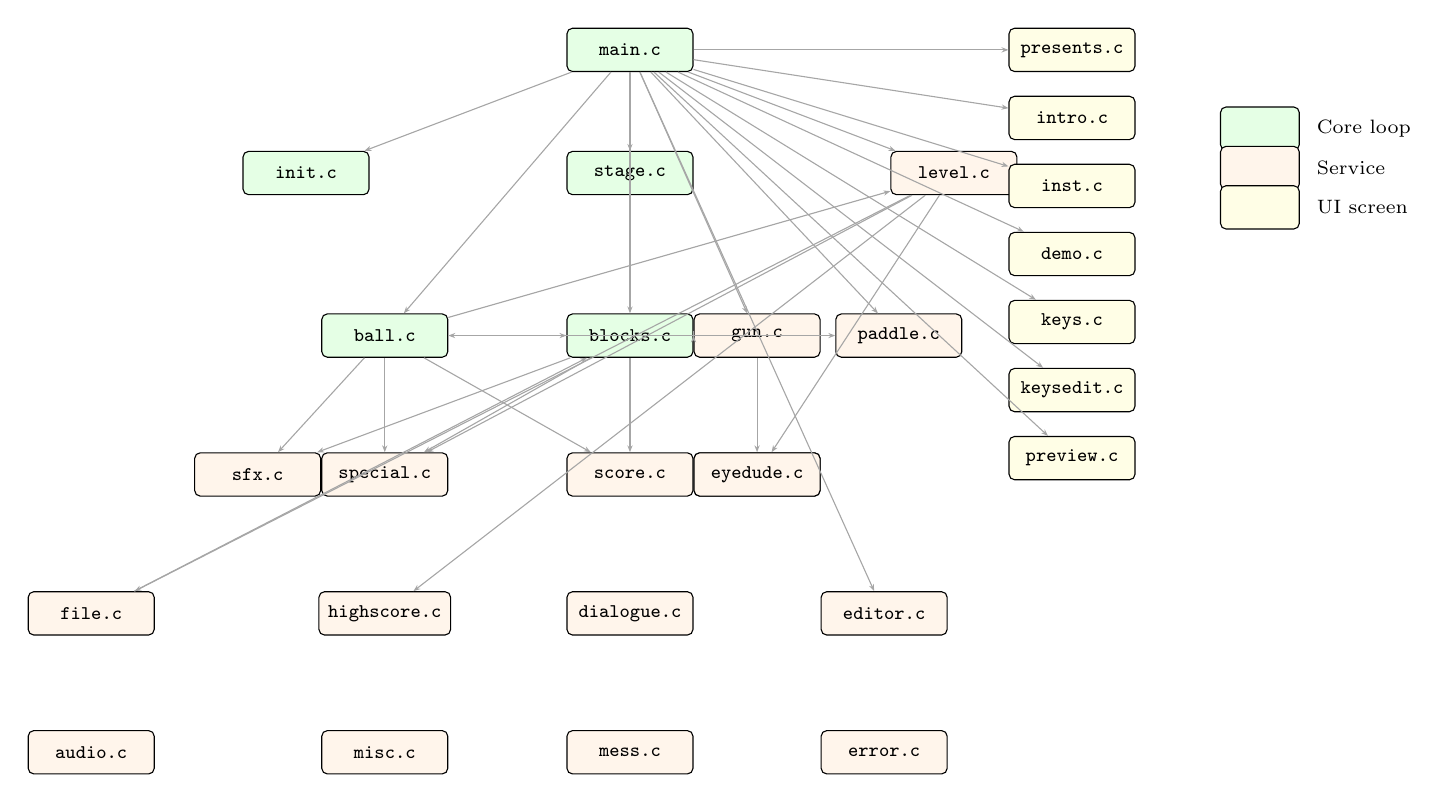
\begin{tikzpicture}[
  mod/.style={draw, rounded corners=2pt, minimum height=0.55cm, minimum width=1.6cm, font=\scriptsize\ttfamily, fill=blue!5},
  core/.style={mod, fill=green!10},
  ui/.style={mod, fill=yellow!10},
  svc/.style={mod, fill=orange!8},
  arr/.style={-{Stealth[length=2.5pt]}, thin, gray!70},
  node distance=0.6cm and 0.9cm,
]
  % Top: main
  \node[core] (main) {main.c};

  % Layer 1: core modules
  \node[core, below left=1cm and 2.5cm of main] (init) {init.c};
  \node[core, below=1cm of main] (stage) {stage.c};
  \node[svc, below right=1cm and 2.5cm of main] (level) {level.c};

  % Layer 2: game logic
  \node[core, below left=1.5cm and 1.5cm of stage] (ball) {ball.c};
  \node[core, below=1.5cm of stage] (blocks) {blocks.c};
  \node[svc, below right=1.5cm and 0cm of stage] (gun) {gun.c};
  \node[svc, below right=1.5cm and 1.8cm of stage] (paddle) {paddle.c};

  % Layer 3: systems
  \node[svc, below left=1.2cm and 0cm of ball] (sfx) {sfx.c};
  \node[svc, below=1.2cm of ball] (special) {special.c};
  \node[svc, below=1.2cm of blocks] (score) {score.c};
  \node[svc, below right=1.2cm and 0cm of blocks] (bonus) {bonus.c};
  \node[svc, below=1.2cm of gun] (eyedude) {eyedude.c};

  % Layer 4: I/O and services
  \node[svc, below left=1.2cm and 0.5cm of sfx] (file) {file.c};
  \node[svc, below=1.2cm of special] (hscore) {highscore.c};
  \node[svc, below=1.2cm of score] (dialogue) {dialogue.c};
  \node[svc, below right=1.2cm and 0cm of bonus] (editor) {editor.c};

  % Layer 5: utilities
  \node[svc, below=1.2cm of file] (audio) {audio.c};
  \node[svc, below=1.2cm of hscore] (misc) {misc.c};
  \node[svc, below=1.2cm of dialogue] (mess) {mess.c};
  \node[svc, below=1.2cm of editor] (error) {error.c};

  % UI screens (right column)
  \node[ui, right=4cm of main] (presents) {presents.c};
  \node[ui, below=0.3cm of presents] (intro) {intro.c};
  \node[ui, below=0.3cm of intro] (inst) {inst.c};
  \node[ui, below=0.3cm of inst] (demo) {demo.c};
  \node[ui, below=0.3cm of demo] (keys) {keys.c};
  \node[ui, below=0.3cm of keys] (keysedit) {keysedit.c};
  \node[ui, below=0.3cm of keysedit] (preview) {preview.c};

  % Edges from main
  \draw[arr] (main) -- (init);
  \draw[arr] (main) -- (stage);
  \draw[arr] (main) -- (level);
  \draw[arr] (main) -- (ball);
  \draw[arr] (main) -- (blocks);
  \draw[arr] (main) -- (gun);
  \draw[arr] (main) -- (paddle);
  \draw[arr] (main) -- (presents);
  \draw[arr] (main) -- (intro);
  \draw[arr] (main) -- (inst);
  \draw[arr] (main) -- (demo);
  \draw[arr] (main) -- (keys);
  \draw[arr] (main) -- (keysedit);
  \draw[arr] (main) -- (preview);
  \draw[arr] (main) -- (editor);

  % Cross-module calls
  \draw[arr] (ball) -- (blocks);
  \draw[arr] (ball) -- (paddle);
  \draw[arr] (ball) -- (score);
  \draw[arr] (ball) -- (sfx);
  \draw[arr] (ball) -- (special);
  \draw[arr] (ball) -- (level);
  \draw[arr] (blocks) -- (score);
  \draw[arr] (blocks) -- (special);
  \draw[arr] (blocks) -- (sfx);
  \draw[arr] (gun) -- (blocks);
  \draw[arr] (gun) -- (ball);
  \draw[arr] (gun) -- (eyedude);
  \draw[arr] (level) -- (file);
  \draw[arr] (level) -- (bonus);
  \draw[arr] (level) -- (hscore);
  \draw[arr] (level) -- (special);
  \draw[arr] (file) -- (blocks);

  % Legend
  \begin{scope}[shift={(8, -1)}]
    \node[core, minimum width=1cm] at (0, 0) {};
    \node[right, font=\scriptsize] at (0.6, 0) {Core loop};
    \node[svc, minimum width=1cm] at (0, -0.5) {};
    \node[right, font=\scriptsize] at (0.6, -0.5) {Service};
    \node[ui, minimum width=1cm] at (0, -1.0) {};
    \node[right, font=\scriptsize] at (0.6, -1.0) {UI screen};
  \end{scope}
\end{tikzpicture}
\caption{Module dependency graph. Arrows indicate ``calls into'' relationships. \texttt{main.c} dispatches to all modules via the state machine. \texttt{ball.c} is the most coupled module (6 outgoing dependencies). UI screen modules (yellow) share a common pattern: each has a multi-state sequence driven by \texttt{handleGameStates()} in \texttt{main.c}.}
\label{fig:module-deps}
\end{figure}


% ============================================================================
\section{Code Metrics}
\label{sec:metrics}
% ============================================================================

\begin{table}[htbp]
\centering
\caption{Codebase metrics (original source, excluding tests and stubs).}
\label{tab:metrics}
\begin{tabular}{lr}
\toprule
\textbf{Metric} & \textbf{Value} \\
\midrule
Source files (\file{.c})          & 29 (27 + 2 generated) \\
Header files (\file{.h})         & 33 \\
Audio driver files                & 12 \\
Source LOC (excl.\ tests)         & 18,606 \\
Header LOC                        & 2,953 \\
Audio driver LOC                  & 2,882 \\
Total LOC                         & 24,441 \\
\code{extern} declarations        & 62 \\
Game modes                        & 16 \\
Block types                       & 30 \\
Level files shipped                & 83 \\
Sound files                       & 46 \\
XPM bitmap directories             & 11 \\
\bottomrule
\end{tabular}
\end{table}

\subsection{Coupling Characteristics}
\label{sec:coupling}

The codebase exhibits several coupling patterns typical of 1990s C game development:

\begin{description}[style=nextline]
  \item[Global state via \code{extern}] 62 \code{extern} declarations across 33 headers. Key shared globals include: \code{mode}, \code{frame}, \code{gameActive} (main.h); \code{display}, \code{mainWindow}, \code{playWindow}, and all 6 GCs (init.h/stage.h); \code{blocks[][]} array (blocks.h).
  \item[X11 type proliferation] The \code{Display*} pointer is passed to virtually every function. X11 types (\code{Window}, \code{Pixmap}, \code{GC}, \code{Region}, \code{Colormap}) are used directly in game logic rather than abstracted behind an interface.
  \item[Module-as-singleton] Each \file{.c} file uses \code{static} variables for persistent state. This is a form of encapsulation, but it means module state cannot be inspected or reset without calling module-specific functions.
  \item[Initialization order dependency] The 33-step initialization sequence in \file{init.c} has implicit ordering constraints. Reordering steps (e.g., creating GCs before windows) produces segfaults with no compile-time protection.
\end{description}


% ============================================================================
\section{Known Issues and Technical Debt}
\label{sec:tech-debt}
% ============================================================================

The following issues motivated the modernization effort. Each is a factual observation about the legacy codebase, not a design criticism---many were reasonable choices for 1993.

\begin{longtable}{p{3cm}p{10cm}}
\caption{Technical debt inventory with modernization rationale.}
\label{tab:tech-debt} \\
\toprule
\textbf{Issue} & \textbf{Details} \\
\midrule
\endfirsthead
\toprule
\textbf{Issue} & \textbf{Details} \\
\midrule
\endhead

X11 server-side collision & Block collision regions (\code{XPolygonRegion}, \code{XRectInRegion}) are computed on the X server. Game logic should not depend on a display server. Replacing with $\sim$20 lines of client-side triangle math removes this dependency. \\
\midrule

Binary save format & \code{saveGameStruct} is serialized via raw \func{fwrite} with no byte-order conversion and no struct padding protection. Save files are not portable across architectures. \\
\midrule

Binary score format & \code{highScoreEntry} uses \func{htonl}/\func{ntohl} for numeric fields but relies on struct layout for \code{name[40]}. Padding between fields can vary across compilers. \\
\midrule

OSS audio via fork+pipe & The \file{/dev/dsp} device (OSS) is deprecated on modern Linux. The fork+pipe model prevents mixing multiple sounds. Volume control is unimplemented. \\
\midrule

K\&R prototype guards & The original headers wrapped function prototypes in \code{\#if NeedFunctionPrototypes} for K\&R C compatibility ($\sim$200 lines). These guards have been removed from the archived source. \\
\midrule

Compile-time paths & File system paths are baked in via \code{-D} flags. The binary can only run from the repo root unless environment variables are set. Incompatible with FHS installation (\file{/usr/share/}, \file{/usr/games/}). \\
\midrule

Hand-tuned frame timing & \func{sleepSync} multiplies the delay by 300 ($\mu$s factor). This constant was tuned for specific hardware and makes frame timing unpredictable on modern systems. No vsync support. \\
\midrule

Private colormap & The PseudoColor colormap causes color flashing when the window manager switches focus on modern TrueColor displays---the private colormap overwrites colors used by other applications. \\
\midrule

XLFD font dependency & Adobe Helvetica bitmap fonts are disappearing from Linux distributions. The \code{fixed} fallback is visually degraded. \\
\midrule

\func{snprintf}/fixed buffers & All \func{sprintf} calls have been converted to \func{snprintf}, but fixed-size buffers remain throughout. The three \code{-Wno-*} compiler flag suppressions silence warnings about format truncation and unused results from \func{snprintf}. \\
\midrule

No test infrastructure & Zero unit tests, no test framework, no deterministic replay. The only way to verify behavior is manual play-testing. \\
\midrule

62 global variables & Cross-module state is shared via \code{extern} globals. This makes reasoning about state ownership difficult and prevents unit testing individual modules in isolation. \\
\bottomrule
\end{longtable}


% ============================================================================
\appendix
\section{Command-Line Options}
\label{sec:cli-options}

\begin{longtable}{llll}
\caption{Complete command-line option table \specref{1}.}
\label{tab:cli-options} \\
\toprule
\textbf{Option} & \textbf{Argument} & \textbf{Default} & \textbf{Effect} \\
\midrule
\endfirsthead
\toprule
\textbf{Option} & \textbf{Argument} & \textbf{Default} & \textbf{Effect} \\
\midrule
\endhead
\code{-display}      & \code{<name>}    & \$DISPLAY    & X display connection \\
\code{-help}         & ---              & ---          & Print help, exit \\
\code{-usage}        & ---              & ---          & Print usage, exit \\
\code{-version}      & ---              & ---          & Print version, exit \\
\code{-setup}        & ---              & ---          & Print path info, exit \\
\code{-sync}         & ---              & off          & X protocol synchronization \\
\code{-debug}        & ---              & off          & Debug mode \\
\code{-sound}        & ---              & off          & Enable audio \\
\code{-nosfx}        & ---              & SFX on       & Disable visual effects \\
\code{-keys}         & ---              & mouse        & Keyboard paddle control \\
\code{-grab}         & ---              & off          & Grab pointer \\
\code{-noicon}       & ---              & icon on      & Disable custom icon \\
\code{-usedefcmap}   & ---              & private      & Use default colormap \\
\code{-scores}       & ---              & ---          & Print scores, exit \\
\code{-speed}        & \code{<1-9>}     & 5            & Game speed \\
\code{-startlevel}   & \code{<1-80>}    & 1            & Starting level \\
\code{-maxvol}       & \code{<1-100>}   & 0            & Max volume \\
\code{-nickname}     & \code{<name>}    & real name    & Player name (max 20 chars) \\
\bottomrule
\end{longtable}


\section{Initialization Sequence}
\label{sec:init-sequence}

The 33-step initialization order from \func{InitialiseGame} in \file{init.c} \specref{16}:

\begin{enumerate}[label=\arabic*., nosep]
  \item Parse command-line arguments
  \item Open X display
  \item Configure display (sync, error handlers, signals, random seed)
  \item Select color visual (PseudoColor $\to$ DirectColor $\to$ TrueColor)
  \item Create/configure colormap
  \item \func{SetUpAudioSystem} (if audio enabled)
  \item Map named colors (8 colors): \func{InitialiseColourNames}
  \item Create windows: \func{CreateAllWindows}
  \item Create 6 graphics contexts: \func{InitialiseGraphics}
  \item Load 4 fonts (with ``fixed'' fallback): \func{InitialiseFonts}
  \item Set window backgrounds from XPM pixmaps: \func{SetBackgrounds}
  \item \func{InitialiseMessageSystem}
  \item \func{InitialiseBlocks} --- block grid and pixmaps
  \item \func{InitialiseBall} --- ball animation frames
  \item \func{InitialiseBullet} --- gun/bullet pixmaps
  \item \func{InitialiseScoreDigits}
  \item \func{InitialiseLevelInfo} --- level info display
  \item \func{InitialisePaddle} --- paddle pixmaps
  \item \func{InitialiseDialoguePixmaps}
  \item \func{InitialiseEyeDudes}
  \item \func{SetUpPresents}
  \item \func{SetUpKeys}
  \item \func{SetUpKeysEdit}
  \item \func{SetUpInstructions}
  \item \func{SetUpIntroduction}
  \item \func{SetUpBonus}
  \item \func{SetUpHighScore}
  \item Create color cycling arrays (\code{reds[7]}, \code{greens[7]})
  \item Display initial level info and time
  \item Draw specials panel
  \item Select input events on main and play windows
  \item Map main window
  \item Install colormap
\end{enumerate}

Shutdown (\func{ShutDown}) reverses this sequence: free all module resources, free GCs, release fonts, free colormap, close display.


\section{Resource Lifecycle Pairs}
\label{sec:resource-lifecycle}

\begin{longtable}{lll}
\caption{Setup/Free function pairs for all modules \specref{16}.}
\label{tab:lifecycle} \\
\toprule
\textbf{Module} & \textbf{Setup} & \textbf{Free} \\
\midrule
\endfirsthead
\toprule
\textbf{Module} & \textbf{Setup} & \textbf{Free} \\
\midrule
\endhead
Audio        & \func{SetUpAudioSystem}          & \func{FreeAudioSystem} \\
Stage        & \func{CreateAllWindows}          & \func{FreeBackgroundPixmaps} \\
Blocks       & \func{InitialiseBlocks}          & \func{FreeBlockPixmaps} \\
Ball         & \func{InitialiseBall}            & \func{FreeBall} \\
Gun          & \func{InitialiseBullet}          & \func{FreeBullet} \\
Score        & \func{InitialiseScoreDigits}     & \func{FreeScoreDigits} \\
Level        & \func{InitialiseLevelInfo}       & \func{FreeLevelInfo} \\
Paddle       & \func{InitialisePaddle}          & \func{FreePaddle} \\
Dialogue     & \func{InitialiseDialoguePixmaps} & \func{FreeDialoguePixmaps} \\
EyeDude      & \func{InitialiseEyeDudes}        & \func{FreeEyeDudes} \\
Presents     & \func{SetUpPresents}             & \func{FreeAllPresents} \\
Keys         & \func{SetUpKeys}                 & \func{FreeKeyControl} \\
KeysEdit     & \func{SetUpKeysEdit}             & \func{FreeKeyEditControl} \\
Instructions & \func{SetUpInstructions}         & \func{FreeInstructions} \\
Introduction & \func{SetUpIntroduction}         & \func{FreeIntroduction} \\
Bonus        & \func{SetUpBonus}                & \func{FreeBonus} \\
HighScore    & \func{SetUpHighScore}            & \func{FreeHighScore} \\
Messaging    & \func{InitialiseMessageSystem}   & \func{FreeMessageSystem} \\
Editor       & \func{SetUpEditor}               & \func{FreeEditor} \\
Misc         & (loaded in init.c)               & \func{FreeMisc} \\
Graphics     & \func{InitialiseGraphics}        & \func{ReleaseGraphics} \\
Fonts        & \func{InitialiseFonts}           & \func{ReleaseFonts} \\
\bottomrule
\end{longtable}


\end{document}
